PREESM is a rapid prototyping framework for multi-core development. For understanding the OpenEM framework a way to construct comparable programs with different multi-core runtime was needed. PREESM provides a way to quickly construct multi-core applications for PC as well as for the Texas Instruments multi-core DSP used in the experiments. In this chapter the PREESM framework is introduced. First, an overview of the framework is given in subsection \ref{subsec:preesm-overview}. Second, the framework overview, the internal representations used by the framework are described in subsection \ref{subsec:preesm-internal}. Third, scheduling in the PREESM framework is explained in subsection \ref{subsec:preesm-scheduling}. And Finally, the code generation in PREESM is explained in subsection~\ref{subsec:preesm-codegen}.

\subsection{PREESM Overview}
\label{subsec:preesm-overview}
PREESM is a collection of tools for rapid prototyping multi-core applications. The tools include a graphical editor for the hardware and the software models, code generators for multiple hardware platforms and an automated generator for fixed schedules. The PREESM tools are used through the Eclipse IDE based environment available at~\cite{preesm}.

In PREESM prototypes of applications are constructed by combining hardware and software models with manually created source code and automatically generated schedule. The software model used in PREESM is based on dataflow models of computation and it is discussed in detail in subsection \ref{subsubsec:preesm-algorithm}. To create a software model in PREESM the application is divided into actors. The actors contain manually created code, which is often written in side-effect free style to enable parallel execution of the actors, but this is not enforced by the framework. The graphical editor for the software model allows the user to create actors and connect them together using first in first out queues.~\cite{preesm}

The model of the target hardware platform is created using a similar graphical tool as the software model. The hardware model is described in subsection \ref{subsubsec:preesm-hardware}. PREESM parses the graphs of the models and creates a static schedule for the executable. The schedule, the actor implementations and the graphs are inputs for the code generator, which creates the multi-core executable.~\cite{pelcat2014preesm} The graphical tools allow the PREESM user to create dependencies between the actors. They also allow a more fine grained control over the code generation by setting estimated actor execution times and selecting the cores on which each actor is allowed to execute.

\begin{figure}[h!]
    \begin{center}
        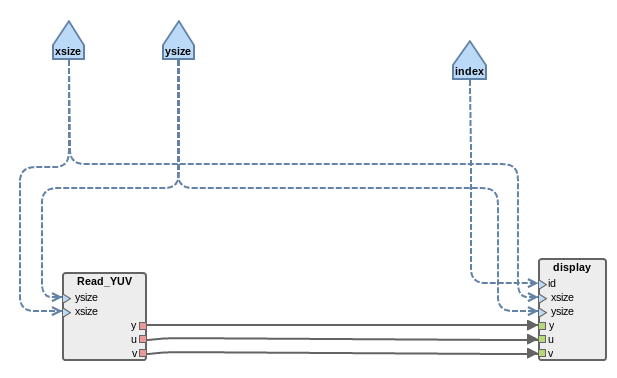
\includegraphics[width=0.99\textwidth]{images/example_preesm_diagram.png}
        \caption{A simple dataflow diagram created with PREESM.}
        \label{fig:preesm_example}
    \end{center}
\end{figure}

\subsection{PREESM Internal Representations}
\label{subsec:preesm-internal}
PREESM applications are created by combining inputs of two different internal representations and manually created source code. The PREESM internal representations are described in this subsection. First, a look is taken at the PREESM algorithm representation PiSDF and second, to the PREESM hardware model.

\subsubsection{PREESM Algorithm Representation}
\label{subsubsec:preesm-algorithm}
In PREESM the applications are modeled using a synchronous dataflow based representation of the software called parameterized and interfaced synchronous dataflow model of computation (PiSDF)~\cite{pelcat2014preesm}. PREESM provides graphical tools for editing the dataflow diagram. An example of an dataflow diagram created in PREESM is presented in figure \ref{fig:preesm_example}. The biggest benefit of using synchronous dataflow based model of computation is that deadlock free static schedules can be generated from them~\cite{pelcat2014preesm}. The static schedules generated by PREESM are guaranteed to be deadlock free~\cite{preesm}.

Dataflow models of computation are a directed graphs where each node represents a function and the arcs are the only possible paths the data can traverse the graph. In the generic dataflow MoC the number of tokens produced or consumed by an actor is not known before execution. For example an actor may have two output paths and it may choose to produce an output token conditionally to either one of the paths. In contrast with the generic dataflow MoCs, in synchronous data flow (SDF) MoC each actor produces and consumes a pre-determined number of tokens. \cite{lee1987synchronous} A more thorough explanation of dataflow MoCs can be found in \cite{lee2015introduction}.

PREESM uses an extended version of SDF called PiSDF \cite{pelcat2014preesm}. PiSDF extends SDF by providing hierarchical graphs based on interfaces and by introducing parameterized actors. An actor in PiSDF can be replaced by a subgraph, which has input and output interfaces. The interfaces insulate the hierarchy levels in terms of schedulability analysis, meaning that schedules can be generated for the subgraphs without knowledge of the higher level models. The parameters are used to configure the production and consumption rates of the actors.~\cite{desnos2013pimm}

An example of a PiSDF graph is presented in figure \ref{fig:preesm_example}. The parameters of the PiSDF model are presented at the top of the figure as pentagons connected to the actors with dashed lines. The actors have input and output ports for parameters and data. The ports define the input and output interfaces of the actors. The actual data paths are the arcs connecting the actors in the bottom of the figure.

\subsubsection{PREESM Platform Representation}
\label{subsubsec:preesm-hardware}
The PREESM code generation is aware of the target hardware platform. PREESM uses an internal representation called the System-Level Architecture Model (S-LAM) \cite{pelcat2009system} to describe the target architecture. S-LAM is designed specifically to provide architecture models of high abstraction level for rapid prototyping purposes. S-LAM has good expressive power and it is suitable for modeling heterogeneous architectures as a S-LAM can contain different types of computational resources and communication links.~\cite{pelcat2009system} In the PREESM context however, the typical S-LAM models are simple. For example the S-LAM representing the TMS320C6678 used in experiment \ref{sec:firstexperiment} is quite simple consisting of eight c6678 cores connected through shared memory.

In PREESM the user inputs the speeds of the hardware components of the S-LAM and the speeds of the connections between them. This information is used by the PREESM scheduler to generate a static schedule, that takes communication delays and the component speeds into account, trying to minimize the time spent waiting for communication.~\cite{pelcat2009system}

\subsection{PREESM Scheduling}
\label{sec:preesm-scheduling}
Scheduling multi-core applications is not a trivial task, because the execution on a single core is sensitive to what other cores are doing. An unsuccessful schedule may result in the application deadlocking or many other kinds of problems. The approach PREESM takes to overcome the complexity of scheduling multi-core applications is using a highly analysable model of computation PiSDF and creating a static schedule based on it. PREESM uses the \textit{List} and \textit{Fast} scheduling methods described in \cite{kwok1997high} for generating a static schedule for multi-core platforms. Using these methods PREESM is able to generate a static schedule and guarantee that it is deadlock free.

The reason why multi-core applications are created in the first place is the performance increase available through parallelising the execution. To get a performance increase from parallelising the application the scheduler must be able to efficiently utilize the multiple cores. The critical measure of performance can be throughput or latency. The designer of the PREESM scheduler has made a decision to focus on so-called latency dominated systems \cite{pelcat2014preesm}. Latency dominated system is defined in \cite{ghamarian2006throughput} as a system where respecting the latency constraint placed upon the system automatically guarantees the satisfaction of the throughput constraint. In other words in the systems PREESM is designed for, each iteration of the application has to fulfill some latency constraint. Fulfilling this latency constraint yields satisfactory throughput. This frees the PREESM scheduler from considering throughput in the scheduling decisions and yields a simpler schedule. Because the scheduler only considers the latency of the execution, the iterations of the algorithm are not interleaved. Instead, all cores are synchronized between the iterations with a barrier.~\cite{pelcat2014preesm}

The execution of the different iterations of the algorithm is not interleaved by the PREESM scheduler. However, intra-iteration interleaving is supported. In intra-iteration interleaving the actors belonging to the same iteration of the algorithm are executed in parallel. \cite{pelcat2014preesm} An example of the intra-iteration interleaving is given in the software pipelining tutorial available at \cite{preesm}.

The dependencies between the actors are defined by the PiSDF model of the application. These dependencies are enough to generate ordering of the actor firings, but to get an efficient schedule the execution times of the actors are needed. The estimated execution times for each actor are provided by the user. The time required for communication between the actors is approximated from the amount out data to be transferred and the speed of the communication links. The data amounts are defined in the actor model and the communication speeds in the S-LAM. With the actor ordering and the timing information, the framework generates a static schedule. \cite{pelcat2014preesm} PREESM framework visualizes the generated schedule with a gantt chart. An example gantt chart is presented in figure \ref{fig:preesm_gantt}.

\subsection{PREESM Code Generation}
\label{sec:preesm-codegen}
\fixme{explain wtf is going on with the explode and implode stuff \\ how does the preesm inter actor communication work in detail \\ explain preesm memory usage}
